\documentclass{../../slides-style}

\slidetitle{Git, практика}{23.09.2022}

\begin{document}

    \begin{frame}[plain]
        \titlepage
    \end{frame}

    \begin{frame}
        \frametitle{Задача на практику}
        \begin{itemize}
            \item Поделиться на команды по 3-4 человека
            \item Завести себе репозиторий на GitHub, один на команду
            \item Расшарить репозиторий всем участникам
            \begin{itemize}
                \item Settings -> Collaborators -> Add people
                \item Для этого нужно, чтобы у каждого члена команды был аккаунт
            \end{itemize}
            \item Скинуть ссылку на репозиторий в чат курса
            \item Завести внутрикомандный канал общения (любой)
            \item Кому-то одному завести и выложить проект и базовую инфраструктуру
            \item Поделить задачу на подзадачи и начать разработку по Git Flow
            \item Смотреть в чат команды --- я, возможно, буду комментировать происходящее
            \item За 10 минут до конца собираемся и показываем, что получилось
        \end{itemize}
    \end{frame}

    \begin{frame}
        \frametitle{Git Flow, напоминание}
        \begin{center}
            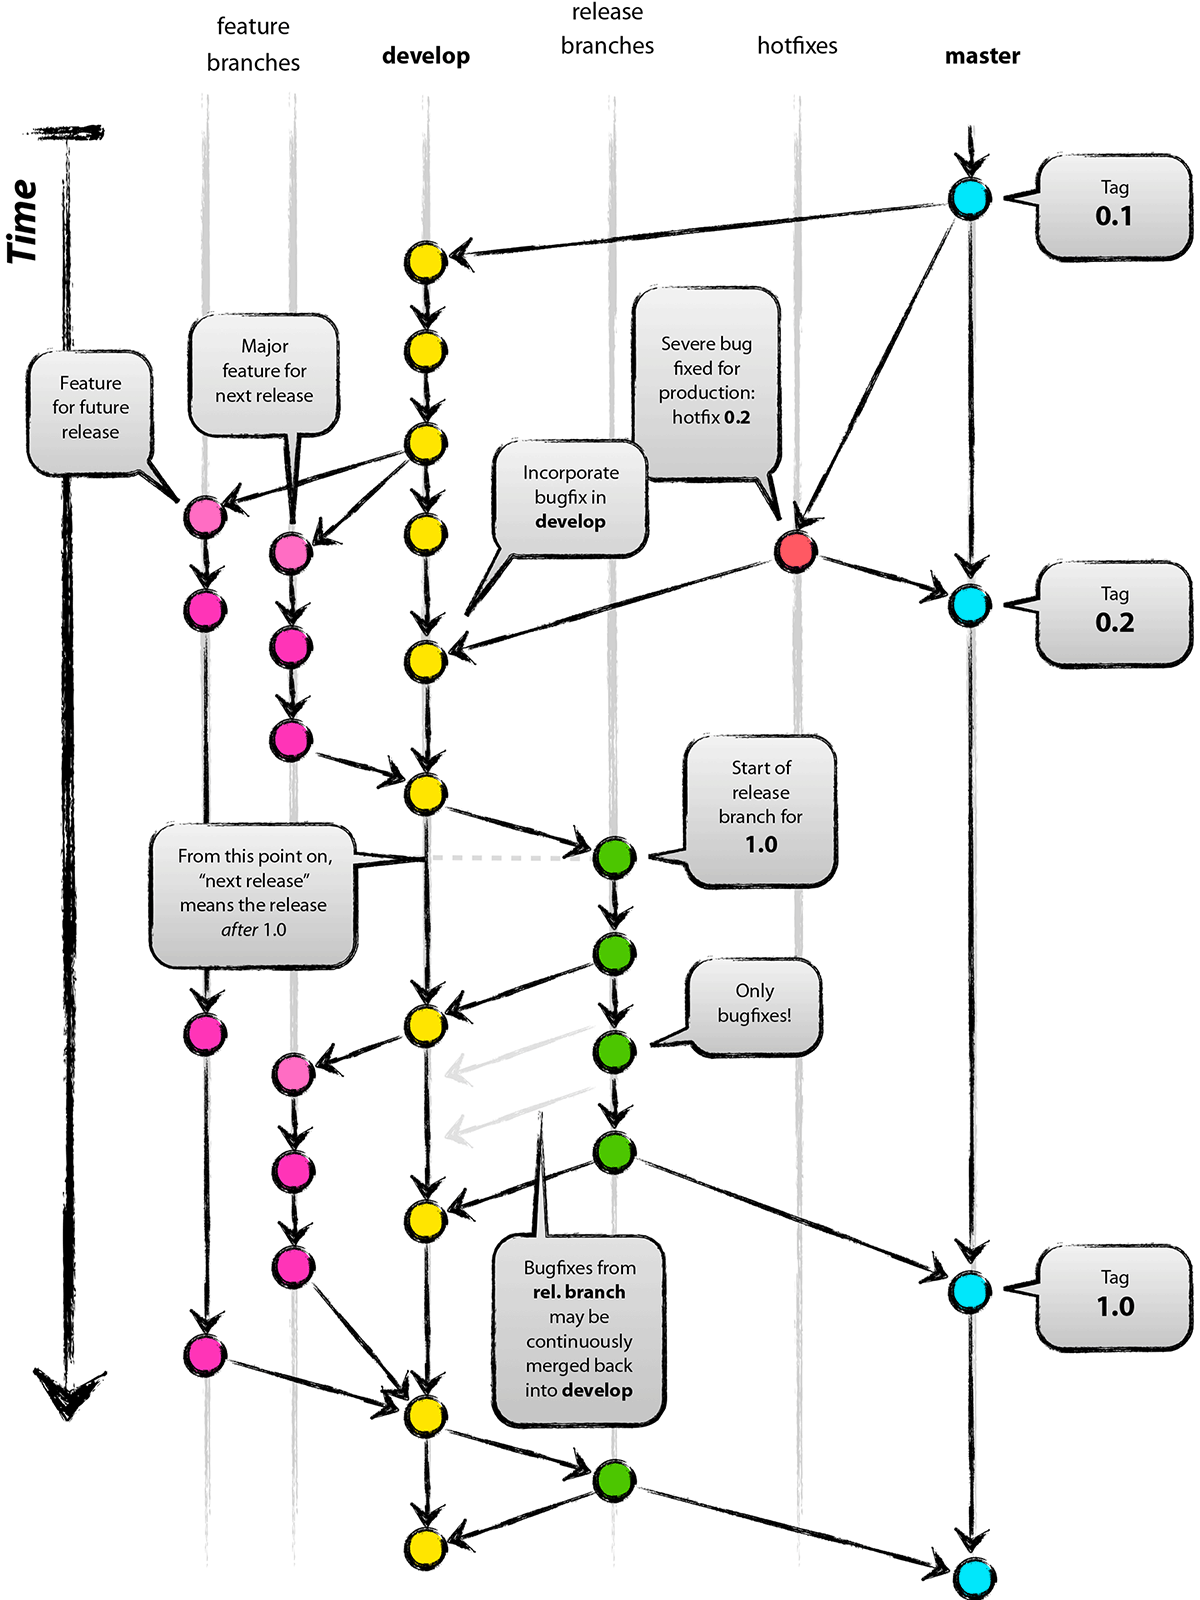
\includegraphics[width=0.42\textwidth]{gitFlow.png}
            \attribution{https://nvie.com/posts/a-successful-git-branching-model/}
        \end{center}
    \end{frame}

    \begin{frame}
        \frametitle{Собственно задача}
        Реализовать список на указателях/ссылках со следующими операциями:
        \begin{itemize}
            \item Insert(int, object) --- добавить элемент по заданному индексу (индексация с нуля, Insert(0, ...) --- добавление в голову)
            \item RemoveAt(int) --- удалить элемент по заданному индексу
            \item Get(int) --- получить элемент по заданному индексу (если ваш язык поддерживает переопределение квадратных скобок, используйте их)
            \item Set(int, object) --- установить элемент по заданному индексу
            \item int Find(object) --- найти индекс по значению
            \item int Count() --- узнать размер списка
            \item Clear() --- очистить список
        \end{itemize}
        Также реализовать для списка итератор. Использовать генерики, если умеете.
    \end{frame}

\end{document}
